%\begingroup
\setlength{\tabcolsep}{-2pt}
%\renewcommand{\arraystretch}{1} % Default value: 1
\begin{table*}[!h]
%\centering
\begin{tabular}{|P{1.1cm}|P{1.1cm}|P{2.7cm}|P{1.3cm}|P{1.3cm}|P{1.5cm}|P{2cm}  N  R|P{6cm}|}
\hline
Nodes & MPI & Dimensions & Interval & Sim$_{cycle}$ & Particles & Memory & Step & DAV\% & Scatter Plots\\ 
 & Ranks & & & & /Node & /Node (MB) & & & \\ 
\hline
%\multicolumn{9}{l}{} & \\
\multicolumn{9}{l}{\textbf{          Cloverleaf3D Proxy Hydrodynamics Application }} & \multirow{13}{*}{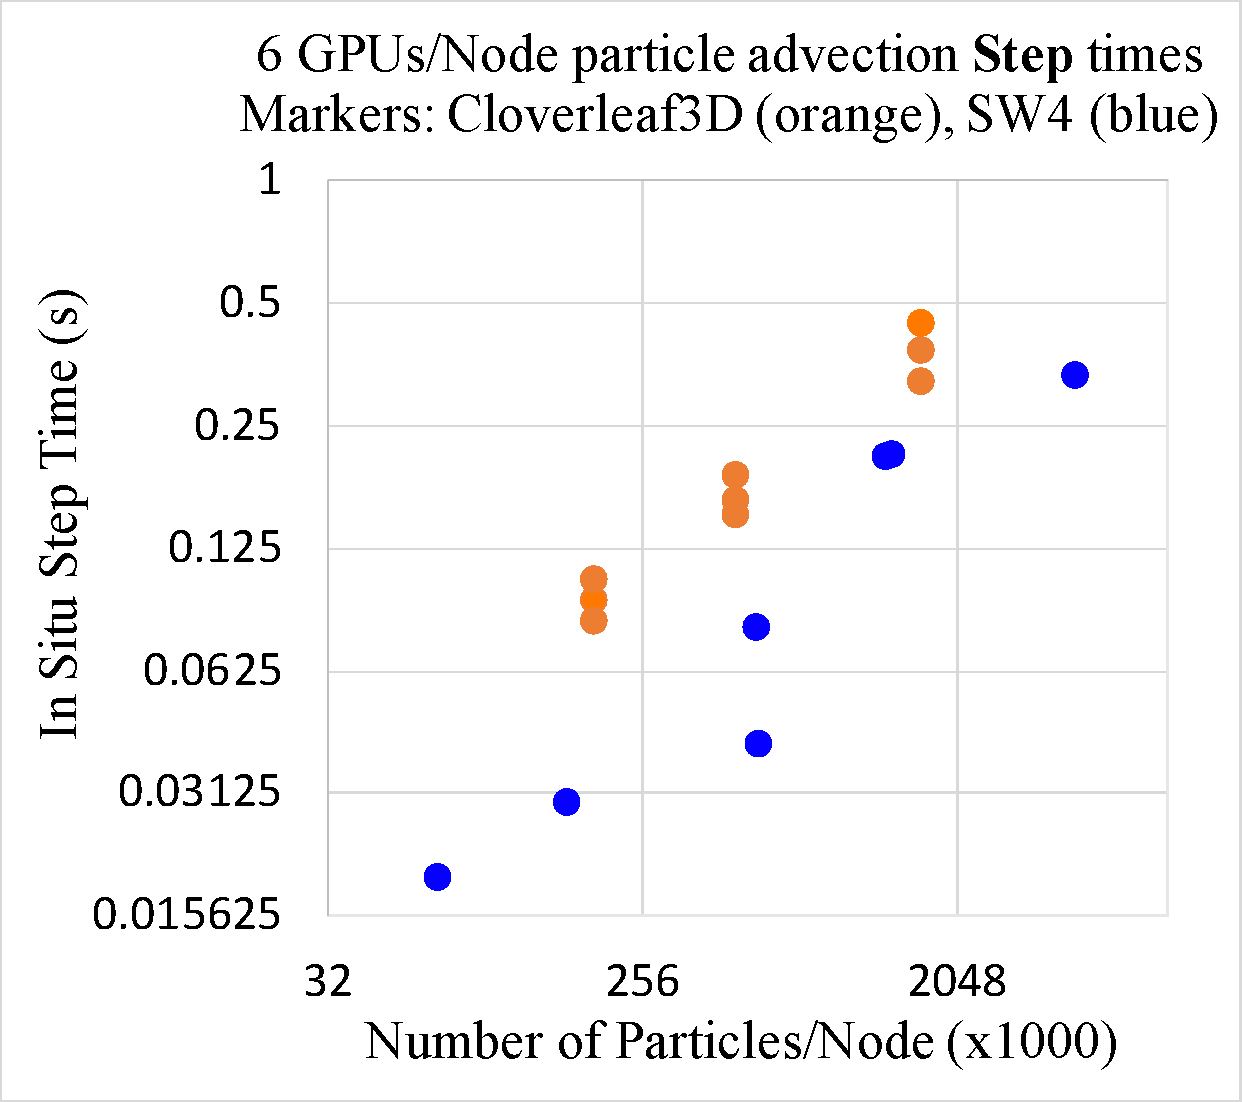
\includegraphics[width=0.93\linewidth]{images/GPU_Step.pdf}}\\
\cline{1-9}
\multirow{9}{*}{16} & \multirow{9}{*}{96} & \multirow{9}{*}{$586\times586\times586$} & 20 & 4.73 & \multirow{3}{*}{1.5M} & \multirow{3}{*}{40.2 } & 0.4475 & 9.408 & \\
\cline{4-4}
& & & 40 & 4.08 & & & 0.3221 & 7.894 & \\
\cline{4-4}
& & & 60 & 4.39 & & & 0.3838 & 8.742 & \\
\cline{4-6}%\cline{6-6}
& & & 20 & 4.50 & \multirow{3}{*}{474k} & \multirow{3}{*}{12 } & 0.1882 & 4.182 & \\
\cline{4-4}
& & & 40 & 4.14 & & & 0.1628 & 3.932 & \\
\cline{4-4}
& & & 60 & 4.33 & & & 0.1498 & 3.459 & \\
\cline{4-6}%\cline{6-6}
& & & 20 & 4.19 & \multirow{3}{*}{186k} & \multirow{3}{*}{4.2 } & 0.0925 & 2.207 & \\
\cline{4-4}
& & & 40 & 4.11 & & & 0.1043 & 2.537 & \\
\cline{4-4}
& & & 60 & 3.87 & & & 0.0830 & 2.144 & \\
\cline{1-9}
%\multicolumn{9}{l}{} & \\
\multicolumn{9}{l}{\textbf{          SW4 Seismic Modeling Simulation }} & \\
\cline{1-9}
\multirow{3}{*}{1} & \multirow{3}{*}{6} & $251\times251\times70$ & \multirow{7}{*}{200} & 0.35 & 555k & 13.89 & 0.0412 & 11.67 & \\
\cline{3-3}\cline{5-6}
& & $335\times335\times93$ & & 2.02 & 1.3M & 33.16 & 0.2125 & 10.48 & \\
\cline{3-3}\cline{5-6}  
& & $501\times501\times139$ & & 7.58 & 4.4M & 111.13 & 0.3309 & 4.365 & \multirow{13}{*}{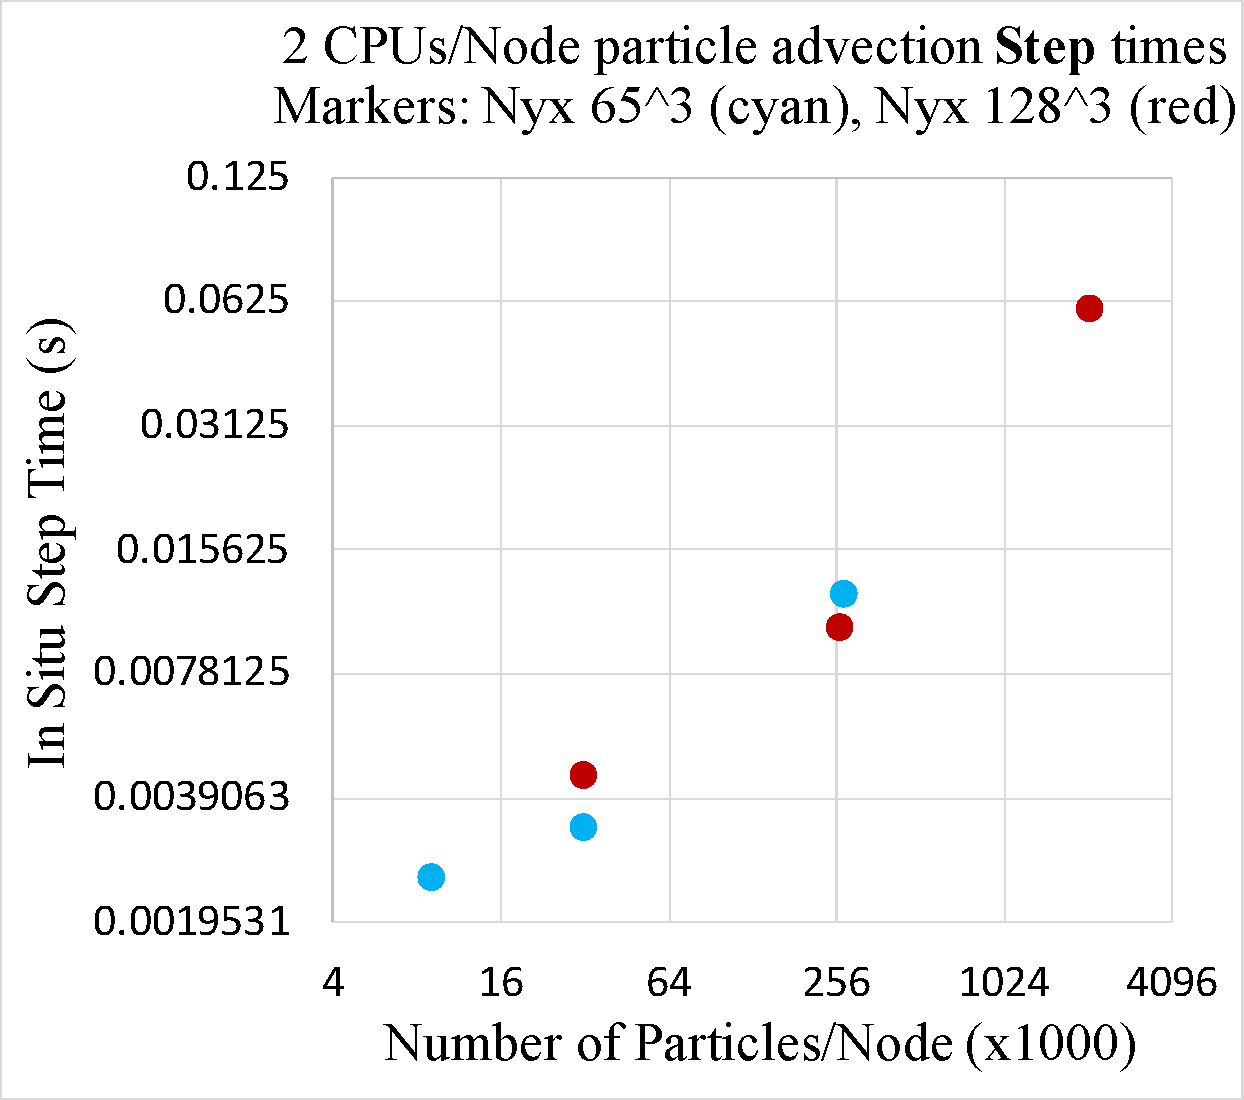
\includegraphics[width=0.93\linewidth]{images/CPU_Step.pdf}}\\
\cline{1-3}\cline{5-6}
\multirow{4}{*}{64} & \multirow{4}{*}{384} & \multirow{3}{*}{$1001\times1001\times276$} & & 1.6 & 66k & 1.6 & 0.0194 & 1.201 &  \\
\cline{6-6}
& & & & 1.5 & 146k & 3.6 & 0.0295 & 1.944 & \\
\cline{6-6}
& & & & 1.3 & 540k & 13.5 & 0.0798 & 6.175 & \\
\cline{3-3}\cline{5-6}
& & $1335\times1335\times368$ & & 2.9 & 1.2M & 31.9 & 0.2095 & 7.074 & \\
\cline{1-9}
%\multicolumn{9}{l}{} & \\
\multicolumn{9}{l}{\textbf{          Nyx Cosmology Simulation }} & \\
\cline{1-9}
\multirow{6}{*}{1} & \multirow{6}{*}{1} & \multirow{3}{*}{$65\times65\times65$} & \multirow{6}{*}{100} & \multirow{3}{*}{10.9} & 274k & 6.8 & 0.0122 & 0.112 & \\
\cline{6-6}
& & & & & 32k & 0.8 & 0.0033 & 0.030 & \\
\cline{6-6}
& & & & & 9k & 0.2 & 0.0025 & 0.023 & \\
\cline{3-3}\cline{5-6}
& & \multirow{3}{*}{$129\times129\times129$} & & \multirow{3}{*}{88.3} & 2.1M & 53.6 & 0.0596 & 0.067 & \\
\cline{6-6}
& & & & & 262k & 6.5 & 0.0101 & 0.011 & \\
\cline{6-6}
& & & & & 32k & 0.8 & 0.0044 & 0.005 & \\
\hline
\end{tabular}
\vspace{-3mm}
\caption{\textit{In situ} encumbrance evaluation and experiment configurations for our three simulation codes.}
\label{table:encumbrance}
\vspace{-5mm}
\end{table*}
\endgroup

Table~\ref{table:encumbrance} contains the results of our experiments for this campaign using all three simulation codes.
%
In this discussion, we assume a simulation can afford to spend 10\% to 20\% on \textit{in situ} processing routines and refer to this as the \textbf{budget}. 
%
Although this might not hold true for every simulation, this estimate is based on interactions with computational scientists and thus, we believe this is a reasonable working estimate.
%
The \textbf{Step} and \textbf{DAV\%} columns in Table~\ref{table:encumbrance} redundantly encode the value in each cell using cell background color (white to pure red hue for the ranges [0,0.75]~(\textbf{Step} in seconds) and [0,20]~(\textbf{DAV\%}), respectively).
%

For \textbf{ISR-2}, i.e., memory costs, we observe that across all experiments, the largest usage of runtime memory was approximately 112 MB.
%
Each Summit node has multiple GBs of memory on CPU~(512) and GPU~(16), and we believe extracting a Lagrangian representation increases the cost of memory on the simulation by approximately one simulation ``field''.
%
We note that simulations can have tens to hundreds of fields defined on the simulation grid and thus, this cost would likely be considered acceptable for most simulations.
%
Our reporting of memory usage is contained in Table~\ref{table:encumbrance}.

\subsubsection{Cloverleaf3D Hydrodynamics Proxy Simulation}
For the Cloverleaf3D simulation, we considered 3 options for number of particles and interval, and 1 option for grid size and concurrency.
%
In particular, we are interested in the \textit{in situ} encumbrance (\textbf{ISR-1}) of varying particle advection workloads, i.e., the number of particles. 
%
We note that each node used 6 GPUs for particle advection and that they all access the same shared memory.
%
For our specific grid size and domain decomposition, each MPI rank operated on over 2M grid points and the Sim$_{cycle}$ was usually between 4-5 seconds. 
%
Overall, we observe an increase in \textbf{Step} costs as the number of particles advected per node increases.
%
Given, the Sim$_{cycle}$ remained relatively stable, the increase in \textbf{Step} is clearly matched by the \textbf{DAV\%} trend.
%

For this integration, we observed that as the number of particles increases from 186k to 474k (2.5X increase) that the cost of performing particle advection only increases by approximately 1.6X. 
%
For the next workload increase, i.e., sampling 1.5M particles ($\sim$3X increase), the cost of performing particle advection increases by approximately 2X.
%
By running the same workload multiple times, we capture variation in the costs within a workload.
%
The variation in the \textbf{Step} cost is greater when the workload is larger and we attribute this to the increased memory allocation and memory transfer costs each step.
%
This is relevant particularly on GPUs where the initial setup cost can be high.
%
%An approximately 0.4\% range in DAV\% across multiple runs using the smallest workload (186k), and up to 1\% variation in DAV\% for the largest workload (1.5M). 
%

Overall, for \textbf{ISR-1}, we found that for our set of experiments increasing the number of particles by 8X results in the \textit{in situ} encumbrance increasing by 3X-4X with the Sim$_{cycle}$ relatively stable.
%
The cost of a single \textbf{Step} to calculate the Lagrangian representation for Cloverleaf3D was as low as 0.08 seconds and in all cases, below half a second, thus, remaining within our identified \textbf{budget}.

\subsubsection{SW4 Seismic Wave Propagation Simulation}
For the SW4 simulation, we considered 2 concurrencies: 1 compute node (6 MPI ranks, GPUs) and 64 compute nodes (384 MPI ranks, GPUs).
%

In the first case, i.e., using 1 compute node and 6 MPI ranks, we considered three grid sizes, each using a proportional number of particles (1:8).
%
We increase the number of particles proportionately, rather than holding it constant, since we believe this would be a more representative of a workload.
%
These results in our empirical study highlight the impact of an increasing grid size on \textbf{ISR-1} and the relation to Sim$_{cycle}$.
%
For the smallest grid size, 555k particles per node are advected every cycle.
%
Although the cost of a particle advection \textbf{Step} is low (0.041s), the \textbf{DAV\%} is over 10\% because the Sim$_{cycle}$ is very small (0.035s) in this case.
%
In contrast, for the largest grid size (each rank operated on 5.8M grid points), we advected 4.4M particles per node and observed a proportional increase in \textbf{Step} cost, but half as much time was spent by the simulation on \textbf{DAV\%}.
%
This is due to the higher Sim$_{cycle}$ for the larger grid size.
%
We note this trend would be expected for computational simulations as they increase in resolution per compute node.
%
%Simulations can require anything between a few seconds to several minutes to complete a cycle.

In the second case, i.e., using 64 compute nodes and 384 MPI ranks, we ran SW4 four times. 
%
Three times with one grid size to observe \textit{in situ} encumbrance for varying particle advection workloads, and one time using a larger grid with 1:8 particles per node.
%
Similar to the Cloverleaf3D experiments, we observed a steady increase in \textbf{Step} and \textbf{DAV\%} as the number of particles per node increases.
%
For the fixed grid size, an 8X increase in the particle advection workload results in an approximately 4X increase, considering Sim$_{cycle}$ with small variability.
%
However, as we increased the grid size, and consequentially, the workload from 540k to 1.2M particles per node ($\sim$2X), although the \textbf{Step} cost increased by over 2.6X, \textbf{DAV\%} increased by less than 1\%.
%

Overall, we first observed that the \textbf{DAV\%} is closely related to the Sim$_{cycle}$. 
%
Although extracting a Lagrangian representation might place a higher encumbrance on a simulation with a small Sim$_{cycle}$ value, for all grid sizes considered the \textit{in situ} encumbrance, i.e., \textbf{DAV\%}, of the corresponding workload remained within our expected \textbf{budget} and the cost of \textbf{Step} was less than half a second in each case.

\subsubsection{Nyx Cosmology Simulation}
Unlike our previous experiments, the Nyx simulation and Lagrangian filter use OpenMP for parallelism, i.e., particle advection is performed using all the CPU cores on a compute node.
%
We considered 3 options for number of particles and 2 options for grid size.
%

First, focusing on the impact of an increase in the grid size on \textbf{ISR-1}, we found a small increase ($<$1.5X) in the absolute cost of a particle advection \textbf{Step} for the same workload, albeit interpolating a grid 8X in size.
%
Further, in the context of \textbf{DAV\%}, the Sim$_{cycle}$ cost increases proportionately to the increase in grid size (8X).
%
Thus, the \textbf{DAV\%} reduces as the simulation grid size increases.
%
Next, for \textbf{ISR-1} across workloads using a fixed grid size, for the smaller grid we observed less than a 5X increase when going from 9k particles to 274k particles per node (30X increase in workload).
%
For the larger grid, a 65X increase in workload resulted in a 13X increase in \textbf{Step} time.

The most interesting finding of these experiments was that using the CPUs, a single particle advection step for the number of particles we considered, costs less than 6 GPUs.
%
For example, the \textbf{Step} cost for 2.1M particles on 2 CPUs is less than half compared to the \textbf{Step} cost for 1.3M and 1.5M particles using 6 GPUs.
%
We do note there are differences, such as 6 GPUs (i.e., 6 MPI ranks) accessing the same memory versus 1 MPI rank on 2 CPUs accessing memory.
%
Although this outcome is likely not surprising (given our knowledge of memory allocation and transfer times for GPUs versus CPUs), this finding certainly encourages future research on how to utilize compute resources if the \textit{in situ} routine frequency is very high (every cycle in our study).
%

Overall, considering the larger Sim$_{cycle}$ times and low memory latency when parallelizing using CPUs, the highest \textit{in situ} encumbrance we observed to extract a Lagrangian representation was 0.1\% of the simulation time.
